\section{Exercise 1}

\section{Answer}
\subsection{1}
Starting from the equation of motion, seen in the equation, we obtain the
state space representation as below:

\[
	A =
	\begin{bmatrix}
		0  	& 		0 		&      1	 	&     0\\
		0 	&     0 		&      0 		&     1\\
		\frac{-(k_1 + k_2)}{m_1} & \frac{k_2}{m_1} & \frac{-c_2}{m_1} & \frac{c_2}{m_1}\\
		\frac{k_2}{m_2} & \frac{-k_2}{m_2} & \frac{c_2}{m_2} & \frac{-c_2}{m_2}
	\end{bmatrix}\quad
	B =
	\begin{bmatrix}
		0\\
		0\\
		\frac{1}{m_1}\\
		0
	\end{bmatrix}\quad
	C =
	\begin{bmatrix}
		1   &  0   &  0  &   0
	\end{bmatrix}
\]

\subsection{2}
Setting \(u\,=\,0\) through the help of the \emph{sdpt3} solver the solution
was solved numerically, obtaining the solution from the Lyapunov inequality for
 \(\mathbf{P}\) given in the matrix \eqref{eq:valuep} is obtained.
 \begin{equation}
 	\label{eq:valuep}
 	\begin{bmatrix*}[l]
 		603.3417	&   -8.5265	&    0.1252	&   -5.0157\\[5pt]
		-8.5265	&  128.7847	&    2.8368	&    0.6276\\[5pt]
		0.1252	&    2.8368	&    3.9082	&    0.5233\\[5pt]
		-5.0157	&    0.6276	&    0.5233	&    1.1363
	\end{bmatrix*}
\end{equation}

\subsection{3}
Using the LMI formulation and using the \emph{sdpt3} solver the \(\mathcal{L}_{2}\)
value of the \(\gamma\) system is estimated.
Where the minimum value assumed by \(\gamma\) is \num{0.5456e-3}.
Moreover, the same result was obtained using the matlab toolbox.

\subsection{4}
From the calculation of the transfer matrix \eqref{eq:tf}, calculated in, we
obtain the Bode diagram in the figure \ref{fig:bodeplot}, where we can see that
the peak has a value of \num{0.5456e-3}.
\begin{align}
	\label{eq:tf}
	\begin{split}
		G(s) 	& = \frac{y(s)}{u(s)} = C(sI-A)^{-1}B\\
				& = \frac{0.01 s^2 + 0.02 s + 1.333}{s^4 + 2.3 s^3 + 303.3 s^2 + 300 s + 20000}
	\end{split}
\end{align}
It is observed that the value of \(\mathcal{L}_{2} = \num{0.5456e-3}\)  is
similar to the peak present in the Bode diagram in Figure \ref{fig:bodeplot}.
\begin{figure}[htb]
	\centering
	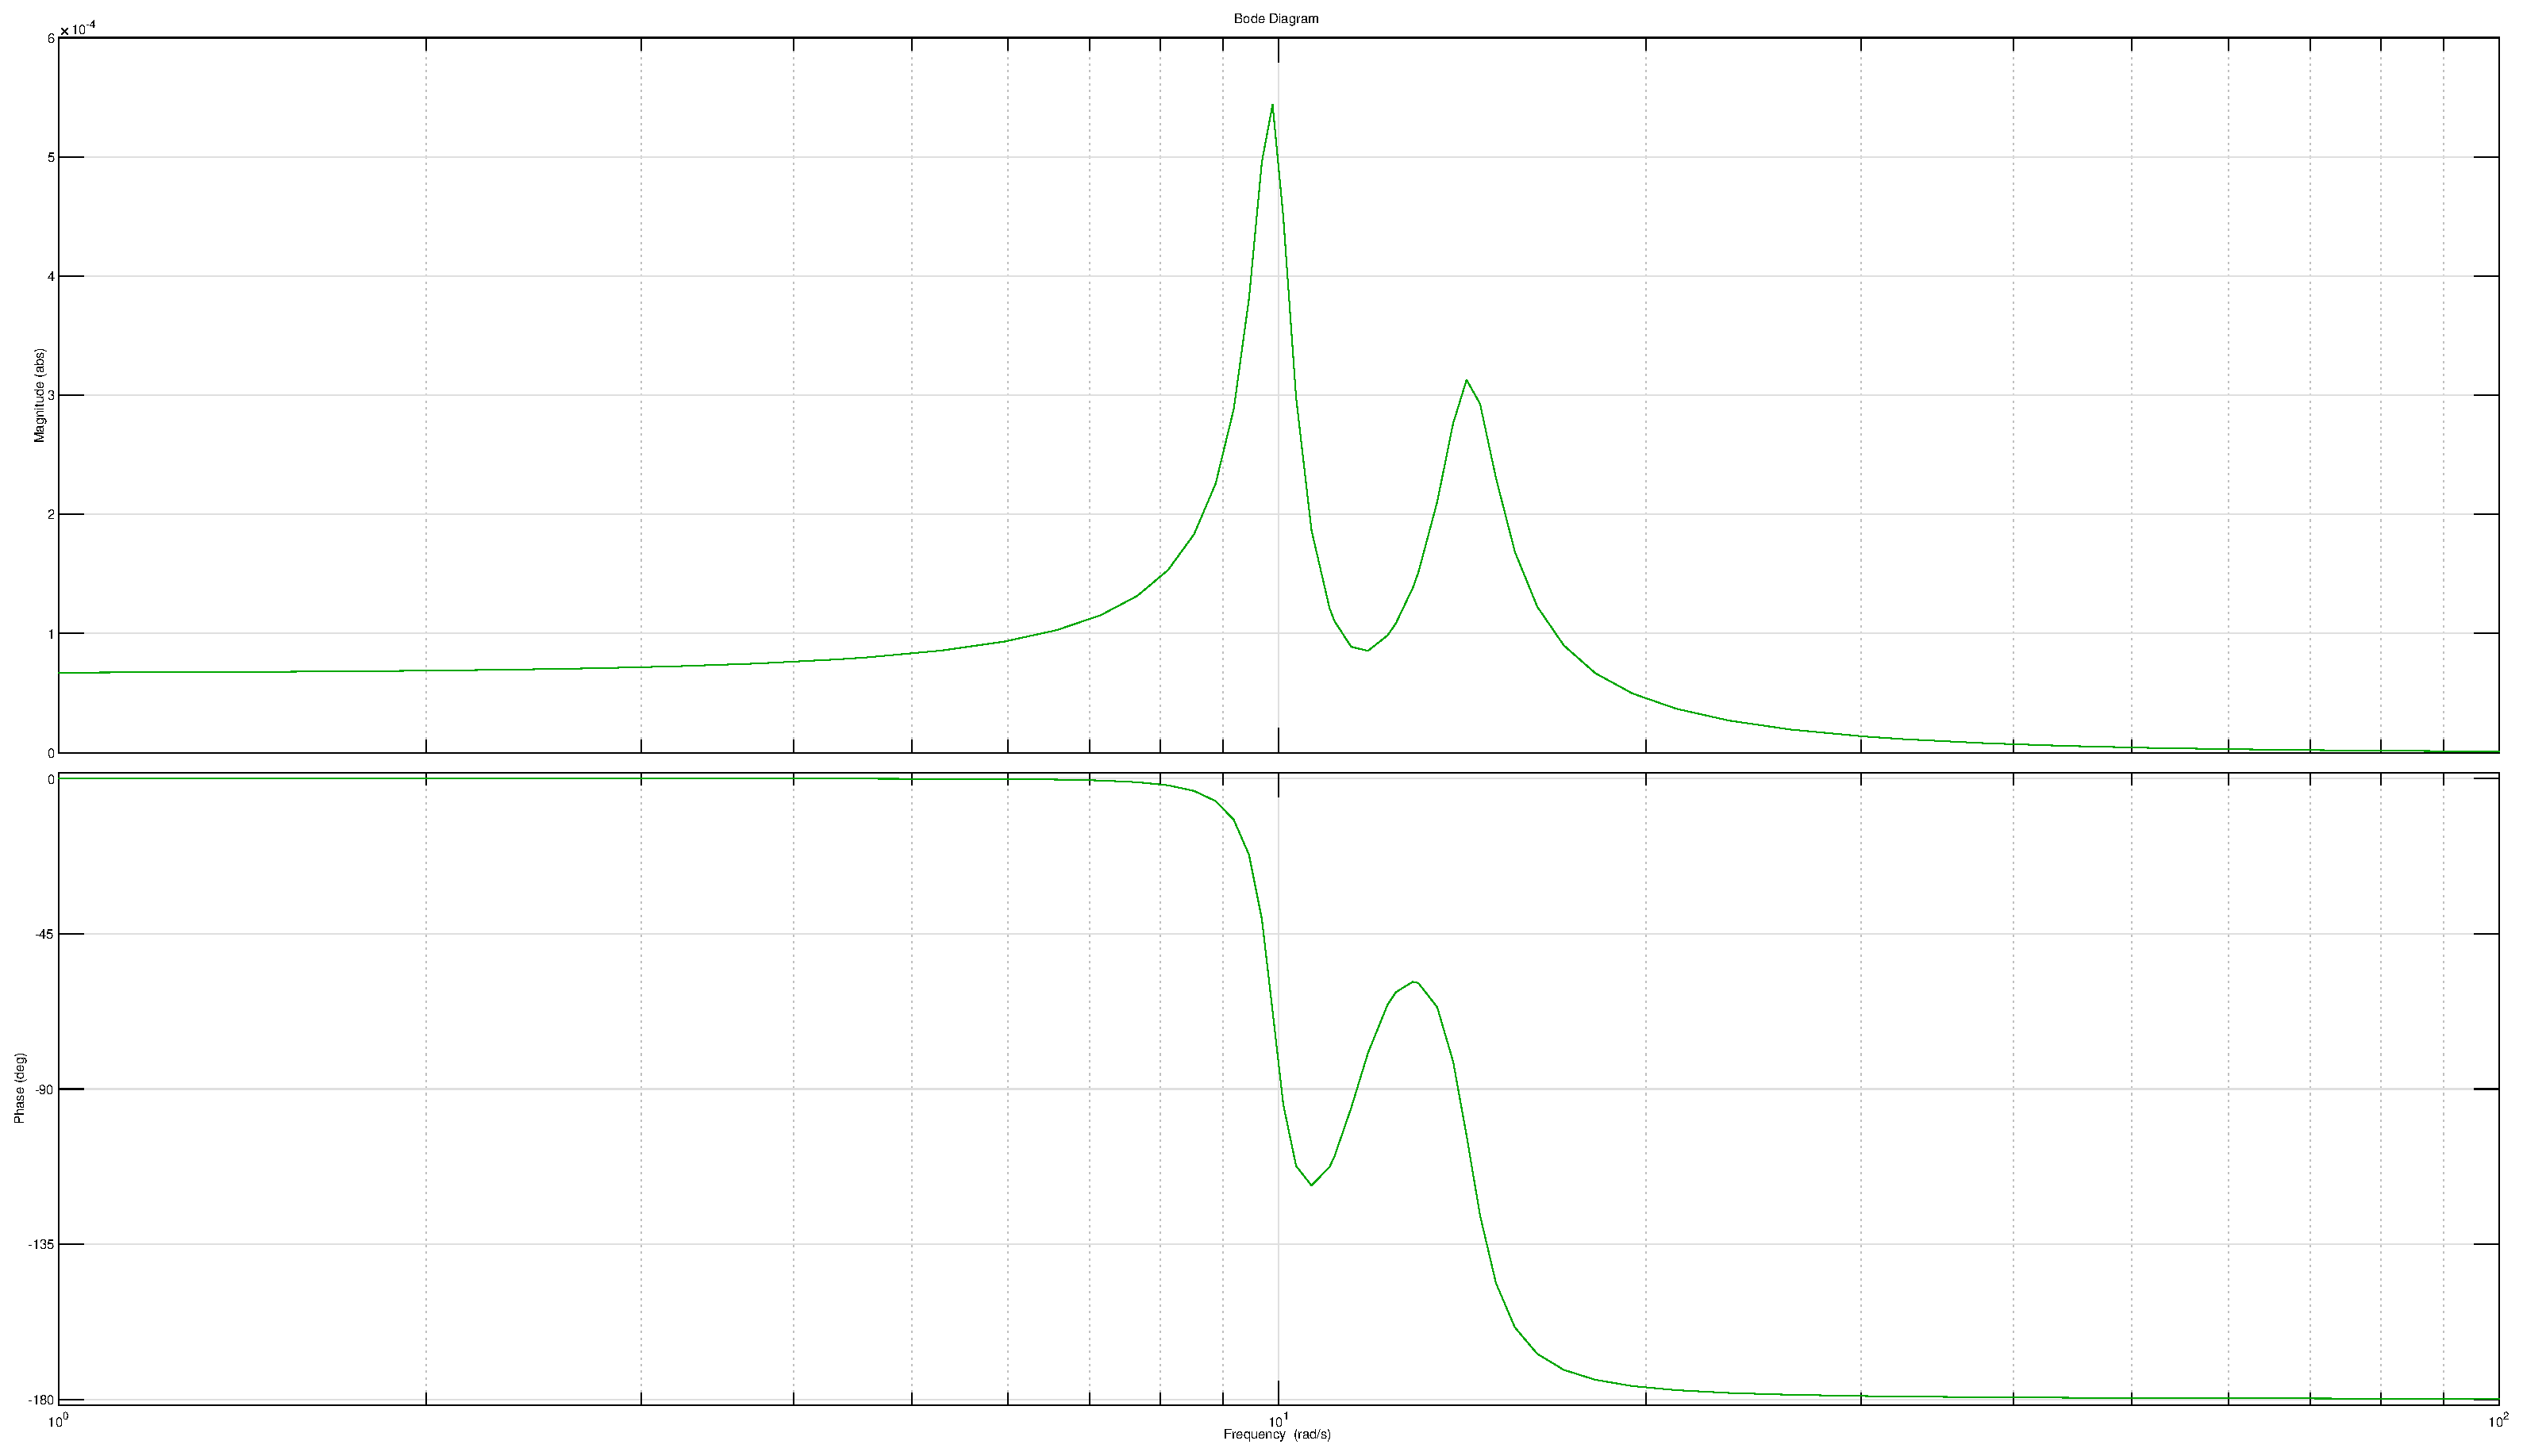
\includegraphics[width=0.75\linewidth]{bode}
	\caption{Bode diagram of tranfer matrix.}
	\label{fig:bodeplot}
\end{figure}
%
\(\mathcal{L}_{2}\) gain is a popular measure of smallness for system
approximation errors and dynamical perturbations.
Consider a causal convolution model of an LTI system, possibly of an
infinite order, defined by the impulse response matrix \(g = g(t)\) or by a
transfer matrix \(G = G(s)\).
Remember that such system defines the output \(y\) as a convolution integral.
\begin{equation}
	\label{eq:convintegral}
	y(t) = \int_{0}^{\infty} h(\tau)f(t-\tau)d\tau
\end{equation}
%
where \(f\) is assumed to vanish fast enough as \(t \rightarrow -\infty\).\\
Let \(\hat{g} = \hat{g}(t)\) and \(\hat{G} = \hat{G}(s)\) be the impulse
response and the transfer matrix of another convolution model, intended to
serve as a simplified approximation of the original one.
One common way of measuring approximation quality is by comparing system
responses \(y_{0} = y_{0}(t)\) and \(\hat{y}_{0} = \hat{y}_{0}(t)\) to a
particular ``testing" input \(f_{0} = f_{0}(t)\).
This leads to the so-called H-Infinity norm of the difference
 \(H(s) = G(s) - \hat{G}(s)\) as the approximation error measure of choice.
